\chapter{Paulions and Gammions}
\label{ch-paulions}

\section{Paulions}

$\vec{a}\in\RR^3$

$\hat{a}= \frac{\vec{a}}{|
\vec{a}|}$

$i=1,2,3$, $\mu=0,1,2,3$

Pauli matrices

\beq
\s_x=\s_1=\left(
\begin{array}{cc}
0&1
\\
1&0
\end{array}
\right),\quad
\s_y=\s_2=\left(
\begin{array}{cc}
0&-i
\\
i&0
\end{array}
\right),\quad
\s_z=\s_3=\left(
\begin{array}{cc}
1&0
\\
0&-1
\end{array}
\right)
\eeq

Hermitian 

\beq
\s_i^\dagger = \s_i
\eeq

Square is 1 (unitary too  because Hermitian)
\beq 
\s_i^2 = 1
\eeq



\beq
\s_x \s_y= -\s_y \s_x 
\eeq
\beq
\s_x \s_y = i \s_z
\eeq

 \beq
\sigma_i \sigma_j = \delta_{ij} I_2+ i \epsilon_{ijk}\sigma_k
\eeq

\beq
\vec{\s}= (\s_1, \s_2, \s_3)
\eeq

\beq
\s_0=\left(
\begin{array}{cc}
1&0
\\
0&1
\end{array}
\right),\quad
\s_\mu = (\s_0, \vec{\s})
\eeq

Suppose $\vec{x}=(x_	1, x_2, x_3)\in\RR^3$. We define the 
{\bf Paulion} $\s_{\vec{x}}$ by\footnote{The term Paulion my own. As far as I know, the construct $\s_{\vec{a}}$,
although often used, doesn't
have a common name.}
\beq
\s_{\vec{x}} = \sigma\cdot \vec{x}=x_1\sigma_1 + x_2\sigma_2 + x_3\sigma_3
\eeq

\begin{claim}

\beq
\s_{\vec{a}}\s_{\vec{b}}=
\vec{a}\cdot\vec{b}+i\s_{\vec{a}\times\vec{b}}
\eeq

With $\vec{a}=\vec{b}$:

\beq
(\s_{\vec{a}})^2 = |\vec{a}|^2 
\eeq

With unit vector $\hat{a}$:
\beq
(\s_{\hat{a}})^2 = 1
\eeq
\end{claim}
\proof
\qed

\begin{claim}
\beq
[\s_{\vec{a}}, \s_{\vec{b}}]_+
= 2(\vec{a}\cdot\vec{b})
\eeq

\beq
[\s_{\vec{a}}, \s_{\vec{b}}]
= 2 i\s_{\vec{a}\times\vec{b}}
\eeq

\end{claim}
\proof
\qed


\begin{claim}
If $\vec{a}\in \RR^3$ then

\beq
e^{i\s_{\vec{a}}}=
\cos |\vec{a}|
+
i \s_{\hat{a}}\sin |\vec{a}|
\eeq
and

\beq
e^{i\beta\s_{\hat{a}}}=
\cos(\beta)
 +i\s_{\hat{a}}\sin(\beta)
\eeq
\end{claim}
\proof

\beq
e^{i
\beta \s_i}=
\cos \beta
+
i \s_i \sin \beta
\eeq
\qed


\begin{figure}[h!]
\centering
\includegraphics[width=2.4in]
{paulions/reflection.png}
\caption{Reflection about plane with normal vector $\hat{a}$}
\label{fig-reflection}
\end{figure}

\begin{figure}[h!]
\centering
\includegraphics[width=2.5in]
{paulions/Rx-pic.png}
\caption{Geometry of $R_{\hat{a}}(\Theta)x$,  where $\Theta=2\theta$}
\label{fig-Rx-pic}
\end{figure}



\begin{claim}
\beq
-\s_{\hat{a}}\s_{\vec{x}}\s_{\hat{a}}=
\sigma_{\rho_{\hat{a}}\vec{x}}
=\av{\s_{\hat{\rva}}}(\vec{x})
\eeq

\beq
\rho_{\hat{a}}\vec{x}=
\vec{x} - 2(\hat{a}\cdot\vec{x})\hat{a}
\eeq
\end{claim}
\proof

\beqa
\s_{\hat{a}}\s_{\vec{x}}\s_{\hat{a}}
&=&
\left[
\hat{a}\cdot\vec{x} + i\s_{\hat{a}\times \vec{x}}
\right]\s_{\hat{a}}
\\
&=&
\hat{a}\cdot\vec{x}\s_{\hat{a}}
+ i 
\underbrace{(\hat{a}\times\vec{x})\cdot\hat{a}}_{=0}
-\s\cdot\underbrace{(\hat{a}\times\vec{x})\times \hat{a}}_{\vec{x}-
(\vec{x}\cdot \hat{a})\hat{a}}
\\
&=&
-\s\cdot\left[\vec{x} - 2(\hat{a}\cdot\vec{x})\hat{a}\right]
\eeqa

\qed


\begin{claim}(Rodrigues formula)

If
\beq
U=e^{-i\frac{\Theta}{2}\s_{\hat{a}}},\quad
\Theta = 2\theta
\eeq
then

\beq
U\s_{\vec{x}}U^\dagger
=
\sigma_{R_{\hat{a}}(\Theta)\vec{x}}
\eeq
where

\beqa
R_{\hat{a}}(\Theta)\vec{x}&=&
\vec{x}
+(2|\vec{x}|\sin\beta\sin\theta)(-\sin\theta \hat{r}+
\cos\theta \hat{\theta})
\\
&=&
\vec{x}
+(2\sin\theta)(-\sin\theta \vec{r}+
\cos\theta \vec{\theta})
\eeqa
where (see Fig.\ref{fig-Rx-pic})

\beq
\beta=\angle(\vec{x}, \vec{a}),\quad
\hat{\theta}=\frac{1}{|\vec{x}|\sin\beta}
\overbrace{(\hat{a}\times\vec{x})}^{\vec{\theta}},\quad
\hat{r}=\frac{1}{|\vec{x}|\sin\beta}
\overbrace{[\vec{x}-\hat{a}(\hat{a}\cdot\vec{x})]}^{\vec{r}}
\eeq

This immediately implies that
$SU(2)_\RR$ is a double cover of $SO(3)$.

\beq
SU(2)_\RR\dmap SO(3),\quad SU(2)_\RR/\{1, -1\} \cong SO(3)\eeq
\end{claim}
\proof

Let $C= \cos \theta$,
$S =\sin \theta$. Then

\beqa
U\s_{\vec{x}}U^\dagger
&=&
(C-iS\s_{\hat{a}})\s_{\vec{x}}(C+iS\s_{\hat{a}})
\\
&=&
C^2\s_{\vec{x}}
-i SC[\s_{\hat{a}}, \s_{\vec{x}}]
+ S^2 
\s_{\hat{a}} \s_{\vec{x}} \s_{\hat{a}} 
\\
&=&
\s\cdot\left\{
C^2\vec{x}
+ 2SC(\hat{a}\times \vec{x})
-S^2[\vec{x} - 2(\hat{a}\cdot\vec{x})\hat{a}]
\right\}
\\
&=&
\s\cdot
\left\{
\vec{x}+2SC\vec{\theta}-2S^2\vec{r}
\right\}
\eeqa



If $U$ produces rotation $R$, then $-U$ gives the same rotation:

\beq
(-U) \s_{\vec{x}} (-U)^\dagger = U\s_{\vec{x}}U^\dagger.
\eeq

\qed










\section{Gammions}

\beq
a\cdot b= a_\mu b^\mu
\eeq

Suppose $a_\mu\in\RR$
for each $\mu$. We define
the {\bf Gammion} $\gamma_\rva$ by\footnote{The term Gammion, like the term Paulion, is my own. As far as I know, the construct $\gamma_\rva$, although often used, doesn't
have a common name.}


\beq
\gamma\cdot a = \gamma_\mu a^\mu = \gamma_\rva
\eeq
We will use an underline in $\gamma_\rva$ 
to distinguish $a$ from an index.


\beq
[\gamma_\mu,\gamma_\nu]_+=2\eta_{\mu\nu}
\eeq

with $\eta_{\mu\nu}$ equals Euclidean $(1,1,1,1)$ or Lorentzian $(1, -1,-1,-1)$ metric.


\beq
\gamma_\rva \gamma_\rvb
= a\cdot b + \gamma_{\mu\nu} a^\mu b^\nu,
\eeq
where bivector

\beq
\gamma_{\mu\nu}=\frac{1}{2}[\gamma_\mu,\gamma_\nu]
\eeq
is the generator of $\mathfrak{so}(n)_\RR$ or $\mathfrak{so}(p,q)$.


A rotation by  $\omega_{\mu\nu}$   is

\beq
S(\omega)=e^{\;\omega^{\mu\nu}\gamma_{\mu\nu}}
\eeq

\beq
 S \gamma_\rvx S^\dagger = \gamma_{Rx}
\eeq
where $R\in SO(n)$ (or $SO(p,q)$).
 
\section{$Spin(n)_\RR$}

%Mathematicians use $Cl(n)_\RR$, $Pin(n)_\RR$, $Spin(n)_\RR$ to mean
%$Cl(n; \FF)$, $Pin(n)_\FF$, $Spin(n)_\FF$ with $\FF=\RR$
%but some people,
%especially physicists, use it to
%mean the \qt{complexified} versions 
%with $\FF=\CC$.
%To avoid confusion,
%here we will
%write the field $\FF$ explicitly.
%In Quantum Mechanics, we use
%$Spin(n)_\CC$. 

If $\gamma_\mu^\dagger=\gamma_\mu$
for $\mu=1,2,\ldots,n$
\beq
Spin(n)_\RR=
\{e^{\omega^{\mu\nu}\gamma_{\mu\nu}}|
\omega_{\mu\nu}=-\omega_{\nu\mu}\in\RR\}
\eeq
If $\gamma_0^\dagger=\gamma_0$, and
$\gamma_i^\dagger=-\gamma_i$ (this assumes the mostly-minus metric $(1, -1, -1, -1)$)
\beq
Spin(1,3)_\RR=
\{e^{-i\omega^{\mu\nu}\gamma_{\mu\nu}}|
\omega_{\mu\nu}=-\omega_{\nu\mu},
\omega_{0,i}\in\RR, \omega_{i,j}
\in i\RR
\}
\eeq

Spinors are the vector space upon which
the group $Spin(n)_\RR$ acts on.


$n_-=n$ for $n$ even and $n_-=n-1$
for $n$ odd.

$e_i\in\RR^n$ for $i=1, 2, \ldots n$. All components
of $e_i$ are zero except the $i$th one.

\beq
\gamma_i=\gamma_{\rve_i}
\eeq

\beq
[\gamma_{i}, \gamma_{j}]_+ = 2 \delta_{i,j}
\eeq

\beq
\Pi_0 = \{1\},
\quad |\Pi_0|={ n \choose 0}=1
\eeq

\beq
\Pi_1=\{\gamma_i|i=1, 2, \ldots, n\}
\quad |\Pi_1|={n\choose 1}=n
\eeq

\beq
\Pi_2=
\{ \gamma_{i_1}\gamma_{ i_2}|i_1<i_2 \},
\quad |\Pi_2|={n\choose 2}
\eeq

\beq
\Pi_3=
\{ \gamma_{i_1}\gamma_{ i_2}\gamma_{i_3}|i_1<i_2<i_3 \},
\quad |\Pi_3|={n\choose 3}
\eeq

\beq
\Pi_{n}=
\{\gamma_1\gamma_2\ldots\gamma_n\},
\quad |\Pi_{2^n}|={n\choose n}=1
\eeq

\beq
\sum_{k=0}^n |\Pi_k| =
\sum_{k=0}^n {n\choose k}= (1+1)^n=2^n
\eeq

\beq
Cl(n)_\RR=span_\RR
\left(\bigcup_{k=0,1,2,\ldots, n}\Pi_k
\right)
\eeq



\beq
Cl^0(n)_\RR = span_\RR
\left(\bigcup_{k=0,2,4,\ldots ,
{n_-}}\Pi_k
\right)
\eeq

\beq
Cl^1(n)_\RR = span_\RR
\left(\bigcup_{k=1,3,5,\ldots ,
{n_-}}\Pi_k
\right)
\eeq

\beq
Cl(n)_\RR= Cl^0(n)_\RR \oplus Cl^1(n)_\RR
\eeq

Since $e^{\omega^{\mu\nu}\gamma_{\mu\nu}}$ is the exponentiation of a bivector, its Taylor expansion only
contains summands with an even number 
of gammas.
\beq
Spin(n)_\RR
\subset Cl^0(n)_\RR
\eeq


\beq
 - \gamma_{\hat{\rva}} \gamma_{\rvx} \gamma_{\hat{\rva}}=
\gamma_{\ul{\rho_{\hat{a}}x}}=
\av{\gamma_{\hat{\rva}}}(x)
\eeq



Fig.\ref{fig-reflection} illustrates reflection about plane with normal vector $\hat{a}$ 
\beq
\rho_{\hat{a}}x
=x - 2(\hat{a}\cdot x)\hat{a}
\eeq

\beq
S^n =\{\hat{a}\in\RR^n| \hat{a}^2=1\}
\eeq

Pin stands for \qt{Product of involutions}
An involution in this case is a unit vector (i.e., $\hat{a}\in \RR^n$ such that
$\hat{a}\cdot\hat{a}=\hat{a}^2=1$) $Pin(n)_\RR$ group
\beqa
Pin(n)_\RR
&=&\cup_{k=1}^\infty
\{
\gamma_{\hat{\rva}_{1}}
\gamma_{\hat{\rva}_{1}}
\ldots
\gamma_{\hat{\rva}_{k}}
| \hat{a}_{i}\in S^n \text{ for all $i$}\}
\eeqa

Note that

One refection
\beq
det[\av{\gamma_{\hat{\rva}}}(x)] = -det(\gamma_\rvx \gamma_{\hat{\rva}}^2)
=-\det(\gamma_{\rvx})
\eeq

Two reflections = a rotation
\beq
det[\av{\gamma_{\hat{\rva}_1}\gamma_{\hat{\rva}_2}}(x)] = +
\det(\gamma_{\rvx})
\eeq

$Pin(n)_\RR$ is a double cover of $O(n)$
(because $det=\pm1$)
\beq
Pin(n)_\RR\dmap O(n), \quad 
Pin(n)_\RR/\{1, -1\}\cong 
O(n)
\eeq

Another definition of $Spin(n)_\RR$ group. This definition
in terms of gammions instead of group generators
\beq
Spin(n)_\RR=\cup_{k=1}^\infty
\{
\gamma_{\hat{\rva}_{1}}
\gamma_{\hat{\rva}_{1}}
\ldots
\gamma_{\hat{\rva}_{{2k}}}
| \hat{a}_{i}\in S^n \text{ for all $i$}\}
\eeq

$Spin(n)_\RR$ is a double cover of $SO(n)$
(because $\av{\gamma_{\hat{\rva}}}=
\av{\gamma_{-\hat{a}}}
$)
\beq
Spin(n)_\RR\dmap SO(n), \quad 
Spin(n)_\RR/\{1, -1\}\cong 
SO(n)
\eeq
\section{Representations of $Spin(n)_\RR$}


Define $Cl(n)_\FF$ is a span over $\FF=\RR,\CC$
and $Spin(n)_\FF\subset Cl^0(n)_\FF$. 

When you go from a vector space
\beq V_\RR =span_\RR(e_1, e_2, \ldots, e_n)\eeq
to \beq V_\CC =span_\CC(e_1, e_2, \ldots, e_n),\eeq this is said to
be a {\bf complexification} of
the vector space. Lie algebras over $\RR$ can be 
complexified. $Cl(n)_\CC$ is the complexification
of  $Cl(n)_\RR$.





$Spin(n)_\RR \dmap SO(n;\RR)$
and 
$Spin(n)_\CC \dmap SO(n;\CC)$.
Rotations by a complex angle as in $SO(n)_\CC$ are meaningless,
even in Quantum Mechanics. 
In Physics, only GROUP
$Spin(n)_\RR$ arises.
However, in Quantum Mechanics,
we use complex representations 
of $Spin(n)_\RR$
and a complex spinor space.
The complex rep of $Spin(n)_\RR$
and the MATRIX SET $Spin(n)_\CC$
are the same thing.

Careful. The following dual 
possibilities are not equivalent
\begin{enumerate}
\item representation of $Spin(n)_\FF$
is real or complex
\item Spinor space on which $Spin(n)_\FF$ acts is real or complex
\item $\gamma$ matrices are real or complex
\end{enumerate}

% Please add the following required packages to your document preamble:
% \usepackage[table,xcdraw]{xcolor}
% Beamer presentation requires \usepackage{colortbl} instead of \usepackage[table,xcdraw]{xcolor}
\begin{table}[h!]
\begin{tabular}{|l|l|l|l|l|l|l|l|l|}
\hline
\rowcolor[HTML]{FFCCC9} 
\cellcolor[HTML]{9AFF99}$n$ & 0 & 1 & 2 & 3 & 4 & 5 & 6 & 7 \\ \hline
\cellcolor[HTML]{9AFF99}{\color[HTML]{000000} $\cong$} & $\RR$ & $\RR\oplus \RR$ & $M_2(\RR)$ & $M_2(\CC)$ & $M_2(\HH)$ & $M_2(\HH)\oplus M_2(\HH)$ & $M_4(\HH)$ & $M_8(\CC)$ \\ \hline
\end{tabular}
\caption{Sets isomorphic ($\cong$) to $Cl(n)_\RR$. In this figure, $M_n(\FF)=\FF^{n\times n}$ for $\FF=\HH, \RR,\CC$ and
$\HH$ are the quaternions.}
\label{tab-bott}
\end{table}

Notes on Table \ref {tab-bott}
\begin{itemize}
\item Dimension check: the real dimension ($dim_\RR$, number of real degrees of freedom, dofs. $dim_\CC= 2dim_\RR$) for the two isomorphic sets is $2^n$ in every case.  For
example, $\dim_\RR M_2(\CC) = 8 = 2^3$ and $dim_\RR(\HH)=4$.
\item The pattern repeats with period 8 (Bott Periodicity). 

\beq
Cl(n+8)_\RR\cong Cl(n)_\RR\otimes M_{16}(\RR)
\eeq
Rather than depending on $n$, they depend on\footnote{In Python $n \mod 8$ is denoted by $n\% 8$,
the remainder after dividing $n$ by 8.}
$n \mod 8$

\item An analogous table for  $Cl(p,q)_\RR$ depends on $(p-q) \%8$

\item 

Complexifying collapses this to the simpler complex classification: 
\beq Cl(2k)_\CC\cong M_{2^k}(\CC) \supset Spin(2k)_\CC\eeq and \beq
Cl(2k+1)_\CC\cong M_{2^k}(\CC)\oplus M_{2^k}(\CC)
\supset Spin(2k+1)_\RR
\eeq
\item For even $n$, $n=2k$,
we can define
a nontrivial  chirality operator:

\beq
\gfive= i^{n/2} \gamma_1\gamma_2\cdots\gamma_n.
\eeq

$\gfive$ satisfies:
\begin{itemize}
\item anticommutes with
all the $\gamma_\mu$

\item commutes with the elements of group $Spin(n)_\RR$
(product of even number of gammas)

\item
$\gfive^2=1$.
\end{itemize}
Therefore it has eigenvalues $1, -1$.
If $S=\CC^{n/2}$,
then

\beq
S = S_+ \oplus S_-,
\eeq
where:

\beq
S_\pm = 
\{\psi \in S \mid \gfive \psi = \pm \psi\}
\eeq
These are the two Weyl (or chiral) spinors in even $n$.


\item For odd $n$, $n=2k+1$,
the expression $\gamma^1\cdots\gamma^n$ is proportional to the identity. Hence,
there is no new operator  that commutes with all the elements of $Spin(n)_\RR$ and there is no
chiral decomposition of vector space $S$.
The space $S$ is irreducible.


\end{itemize}



\section{Examples}
\hrule
$Spin(2)_\RR$

\beq
Cl(2)_\RR=span_\RR \{1, \s_1, \s_2, \s_1\s_2=i\s_3\}
\eeq

\beq
Cl^0(2)_\RR=
span_\RR\{1,\s_1\s_2=i\s_3\}
=\{Ae^{i \theta \s_3}: \theta, A\in\RR\}
\cong\CC
\eeq

\beq
Cl^1(2)_\RR=
span_\RR\{\s_1, \s_2\}
\eeq

\beq
Cl(2)_\RR= Cl^0(2)_\RR \oplus Cl^1(2)_\RR
\eeq

\beq
Spin(2)_\RR=
\{
e^{i\theta\s_3}:
\theta\in\RR\}
\cong U(1)
\eeq



\begin{claim} (Double Cover)

 $Spin(2)_\RR\dmap SO(2)$.
\end{claim}
\proof

Note $U= e^{i\theta \s_3}$ and $\vec{x}= (x_1, x_2)$

\begin{align}
U\s_{\vec{x}}U^\dagger
&=
\left(
\begin{array}{cc}
e^{i\theta} & 0
\\
0 & e^{-i\theta}
\end{array}
\right)
\left(
\begin{array}{cc}
0 & x_1 - i x_2
\\
x_1 + i x_2 & 0
\end{array}
\right)
\left(
\begin{array}{cc}
e^{-i\theta} & 0
\\
0 & e^{i\theta}
\end{array}
\right)
\\
&=
\left(
\begin{array}{cc}
0&z^* e^{i2\theta}
\\
ze^{-i2\theta}&0
\end{array}
\right)  \quad (z = x_1 + i x_2)
\\
&=
\left(
\begin{array}{cc}
0 & x'_1 - i x'_2
\\
x'_1 + i x'_2 & 0
\end{array}
\right)
\end{align}

\beq
x_1' = \Re(ze^{-i2\theta})=
x_1 \cos 2\theta + x_2 \sin \theta
\eeq

\beq
x'_2 = \Im (ze^{-i2\theta})
=
-x_1 \sin 2\theta +
x_2 \cos 2\theta
\eeq

\beq
R_z(2\theta)=
\left(
\begin{array}{cc}
\cos 2\theta & \sin 2\theta
\\
-\sin 2\theta & \cos 2\theta
\end{array}
\right)
\eeq

\beq
\vec{x}= (x_1, x_2)^T,
\quad 
\vec{x'}= (x_1', x_2')^T
\eeq

\beq
\vec{x'}= R_z(2\theta)\vec{x}
\eeq

The 2-1 map:

\beq
e^{i\theta\s_3}\mapsto R_z(2\theta)
\eeq

\qed
\hrule
$Spin(3)_\RR$


\beq
Cl(3)_\RR=span_\RR \{1, \s_1, \s_2, \s_3,\s_1\s_2=i\s_3, i\s_2, i\s_3, \s_1\s_2\s_3=i\}
\cong \CC^{2\times 2}
\eeq

\beq
Cl^0(3)_\RR=
span_\RR\{1,i\s_1, i\s_2, i\s_3\}
\cong \HH
\eeq

\beq
Cl^1(3)_\RR=
span_\RR\{\s_1, \s_2, \s_3, i\}
\cong -i\HH
\eeq

\beq
Cl(3)_\RR= Cl^0(3)_\RR \oplus Cl^1(3)_\RR
\cong \HH \oplus -i\HH
\eeq

\beq
Spin(3)_\RR=
\{
e^{i\s_{\vec{a}}}|\vec{a}\in\RR^3\}
\cong SU(2)
\eeq



\begin{claim}
\beq
SL(2;\CC)\supset SU(2)\cong Spin(3)_\RR\dmap SO(3)\eeq 
\end{claim}
\proof
\qed


\hrule
Quaternions

The set of quaternions is called $\HH$ in honor of Hamilton. ($\QQ$ is already used for the rationals).
A quaternion $q$ is an expression of the form

\beq
q= a + x\mathbf{i}
+ y\mathbf{j}
+
z\mathbf{k}
\eeq
where $a,x,y,z\in\RR$

\beq
i\sigma_1 \leftrightarrow \mathbf{i},\qquad
i\sigma_2 \leftrightarrow \mathbf{j},\qquad
i\sigma_3 \leftrightarrow \mathbf{k}
\eeq

Quaternion multiplication rules
\beq
(i\sigma_i)(i\sigma_j)
= -(\delta_{ij} + i\epsilon_{ijk}\sigma_k)
\eeq

























